\documentclass[a4paper]{proc}

\usepackage{biblatex}
\usepackage{graphicx}

\addbibresource{references.bib}

\renewcommand*{\bibfont}{\raggedright}

\begin{document}

  \title{An analysis of Public Cloud service providers}
  \author{James Robinson\\\texttt{jr4e09@soton.ac.uk}}
  \maketitle

  \begin{abstract}
  \end{abstract}

  % Hypothesis: it's difficult for small companies to get into IaaS because of the associated costs, but building PaaS services on top of existing IaaS ones is feasible with little initial investment.

  \section{The importance of the idea}
  \label{sec:idea}

  % Identify a technology market sector and identify the key players that operate in it.
  %    Market sector: public cloud computing service providers (not software, not private cloud)
  % Identify at least 2 competing products or services and discuss their target customer’s requirements and how these products/services address these needs.
  % You should argue your own opinion as to whether they are successful.
  % It can be useful to research competitors who have failed in the market to provide evidence

  Cloud computing is ``a model for enabling ubiquitous, convenient, on-demand network access to a shared pool of configurable computing resources (e.g., networks, servers, storage, applications, and services) that can be rapidly provisioned and released with minimal management effort or service provider interaction'' \cite{Mell2011}. In essence, it is a tool that allows users to automatically provision computing resources on an on-demand basis, without having to manage the underlying infrastructure.

  The most fundamental type of cloud computing service is known as \emph{Infrastructure as a Service}, or IaaS. IaaS providers offer servers (either physical or virtual) on an on-demand basis, usually charging a fixed price per unit of time the server is used. IaaS providers frequently complement these servers with additional services such as block storage (e.g. virtual disks), object storage (e.g. key-value stores), load balancing, or additional IP addresses, again charging a fixed sum per unit of time the additional services are used. IaaS services are extremely valuable because they abstract away the physical infrastructure (servers, switches, routers, etc.), allow servers to be dynamically provisioned and de-provisioned to meet demand in real-time, and replace the large initial investment for the purchase of physical hardware with smaller incremental payments based on usage.

  A higher-level cloud computing model is known as \emph{Platform as a Service}, or PaaS. PaaS providers offer complete platforms for the deployment of applications, and automatically manage the provisioning of the underlying infrastructure on behalf of the application. This complete platform typically consists of an operating system, a runtime environment for one or more programming languages, libraries, a database server, one or more web servers and a load balancer. PaaS services are extremely valuable because they allow application developers to deploy their application without having to worry about provisioning and maintaining the underlying infrastructure or the software used to host the application.

  Cloud computing can employ a number of different \emph{deployment models} (see figure~\ref{fig:cloud_computing_types}), determined by the entity that owns, controls or manages the underlying hardware \cite{Mell2011}. A \emph{public cloud} service is any cloud service that is provisioned for open use by the general public, regardless of which entity owns or manages it. Due to space constraints, only these services will be considered in this article.

  \begin{figure}
    \centering
    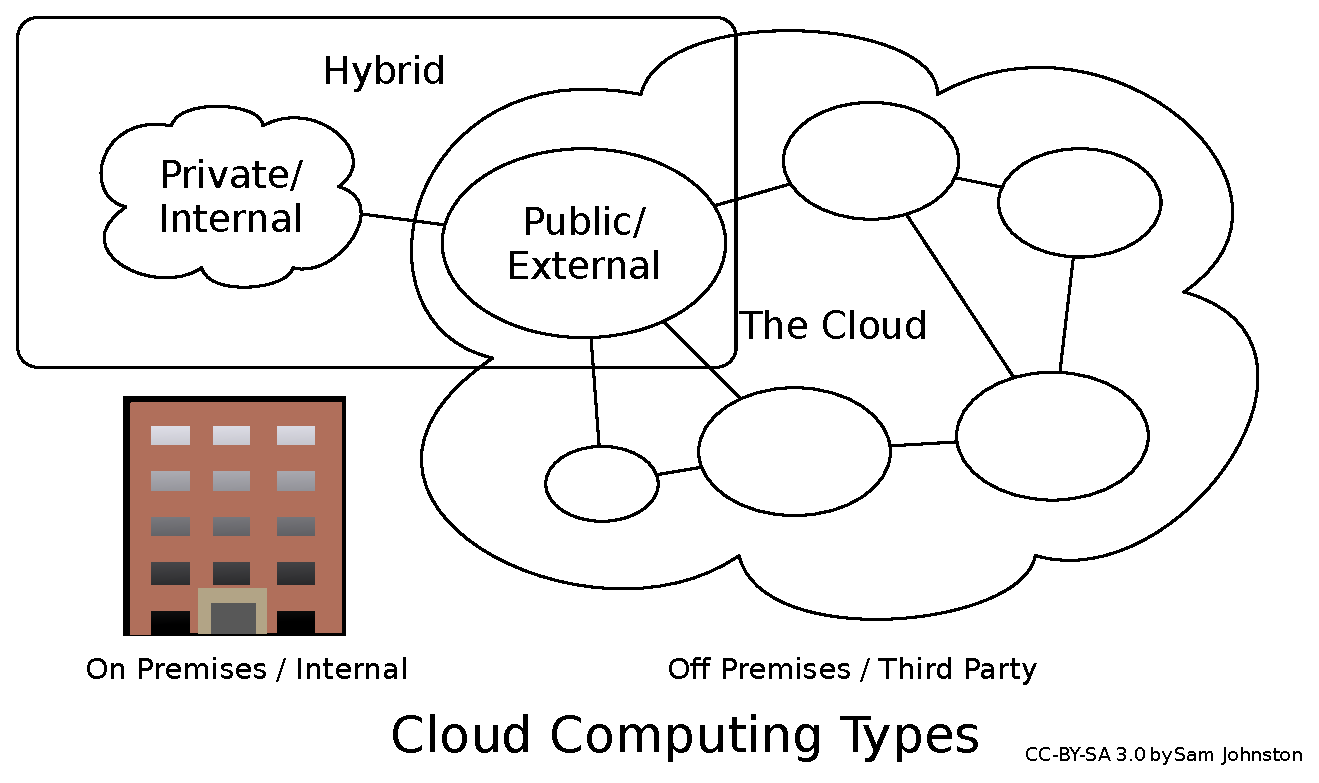
\includegraphics[width=\columnwidth]{figures/Cloud_computing_types.eps}
    \caption{Diagram showing three main types of cloud computing (public/external, hybrid, private/internal) \cite{Joton2009}}
    \label{fig:cloud_computing_types}
  \end{figure}

  Many IaaS providers also offer PaaS services built upon their own infrastructure. An example of such a service is Amazon Web Services (AWS), which provides IaaS in the form of virtual servers (EC2), block storage (EBS), object storage (S3), relational databases (RDS) and load balancing (CloudFront), along with a PaaS (Elastic Beanstalk) that automatically provisions and manages the aforementioned resources as required to run a particular web application. Various languages are supported, including Ruby, PHP, Python, Java and Node.js, but additional fees are incurred for deployment of applications built within Microsoft's software ecosystem, due to licensing requirements. A competitor is Microsoft Azure, which provides both IaaS and PaaS services primarily for applications built upon Microsoft's ecosystem (for example, .NET applications). AWS is an incredibly extensive and popular platform, operating over 1.4 million servers across 28 availability zones as of December 2014 \cite{Mathews2014}.

  Some popular PaaS-only services include Heroku, Red Hat OpenShift, Google App Engine, and Engine Yard. Each of these services can provision and manage the services required to run applications in various popular development ecosystems including PHP, Rails (and other Rack frameworks), Django and Node.js.

  \section{The importance of the market}
  \label{sec:market}

  % Using your original examples (and/or others) explain how market and distribution are important.
  % For example, how big is the market, what strategies are used to access the market
  %   (low price/high volume, free download/in-app purchase, monopolisation, or a platform for 3rd party competition)

  Cloud computing is an enormous market, predicted to reach \$127bn by 2017 \cite{GIA2013}. It is also a highly competitive sector, with companies typically relying on economies of scale to stay afloat. Amazon Web Services, for example, operates on extremely narrow profit margins, relying instead on their extremely high volume of sales to generate income. Their ubiquity in the IaaS market allows them to profit secondarily from PaaS providers built upon their infrastructure. Heroku, a PaaS provider in direct competition with Amazon's own Elastic Beanstalk, relies almost entirely on Amazon's infrastructure.

  \section{Protection}
  \label{sec:protection}

  % Explain why barriers to entry to a market are important, what these barriers can look like eg patents and how companies can protect their ideas and markets.
  % Again you can use your original example companies, or you can introduce new examples.

  The enormous upfront costs associated with purchasing and maintaining the infrastructure needed for an IaaS platform might prove a barrier to entry for smaller companies. Typically the only successful IaaS offerings tend to arise from already-large companies opening up access to their own server infrastructure (e.g. Amazon Web Services, Microsoft Azure). PaaS platforms, on the other hand, are significantly cheaper to run because they can be built upon pre-existing IaaS platforms, allowing PaaS providers to only pay for infrastructure that their clients are actually using. It is likely for this reason that a much larger number of PaaS providers exists.

  An important consideration for PaaS providers in particular is which software ecosystem to provide, including operating system (Windows incurs additional costs over other operating systems but provides access to Microsoft's ecosystem), programming language runtimes, and installed libraries. Providing access to more technologies might increase market reach, but also increase the complexity of maintaining the software builds used on the service.

  \section{Finance}
  \label{sec:finance}

  % Describe how technology companies can be financed and what sort of idea requires what sort of finance.
  % Give examples to support your hypotheses. (Examples might include bank loans, venture capital, crowdfunding, payment in advance from a customer)

  As discussed in section~\ref{sec:idea}, successful IaaS offerings tend to spring from large companies with extensive server infrastructure. Amazon Web Services, for example, begun in an effort to gain revenue from investment in additional infrastructure for the company's main service, Amazon.com \cite{Black2009}. It is extremely difficult for a small company to compete in the IaaS market due to the costs associated with purchasing and maintaining the required infrastructure (on the order of tens of billions of pounds). Currently existing providers operate within extremely tight profit margins, further raising the barrier for entry.

  PaaS providers, on the other hand, can operate on far smaller initial investments since they can rely on IaaS services provided by other companies. Heroku, founded in 2007 on a (relatively) meager initial investment of \$3m \cite{Hendrickson2008}, relies on Amazon Web Services to provide its infrastructure.

  Venture capital can prove an important source of funding for startups in this sector -- Engine Yard, a PaaS provider founded in 2006, secured a total investment of \$37.5m from Benchmark Capital, New Enterprise Associates, Amazon, Bay Partners, Presidio Ventures and DAG Ventures between January 2008 and October 2009 \cite{Schonfeld2008} \cite{Lerner2008}, before receiving an undisclosed strategic minority investment from Oracle Corporation in November 2012 \cite{Oracle2012}.

  \section{Survival}
  \label{sec:survival}

  % What strategies can technology companies use to ensure their survival?
  % Look for examples where companies haven’t survived and maybe should have.
  % Likewise look for examples of companies who are implementing survival strategies

  In order to determine what allows cloud computing providers to survive, it is useful to first consider companies that have failed, and learn from their mistakes. Nirvanix, a cloud storage provider similar to Amazon S3, managed to secure over \$70m in investment since its foundation. It was led by an extremely experienced management team, and boasted more than 1,200 customers in mid 2012. In October 2011, the company entered into a strategic partnership with IBM Global Services. Despite all this financial backing, the company filed for bankruptcy in October 2013. \textcite{Robinson2013} cites 3 primary causes for the company's failure:

  \begin{enumerate}
    \item They charged a flat rate per gigabyte-month for storage, but had to pay inordinate amounts of money for the infrastructure to support the survice. This business model is extremely difficult to support at scale without relying on third-party IaaS providers, especially for a startup.
    \item They didn't own any significant intellectual property rights in their sector; instead, the company's business model relied on its ability to scale to fit the size of the target market, but the price consumers were willing to pay was not enough to sustain the infrastructure.
    \item They didn't branch out into other cloud computing sectors. Competing products like Amazon S3 are popular because they form part of a wider ecosystem, usually providing object storage for applications hosted on Amazon's own EC2 service. Nirvanix provided cloud storage, and nothing else.
  \end{enumerate}

  From this we can infer that a successful cloud computing startup must either outsource infrastructure (for example, by relying on other IaaS proviers for physical infrastructure), or have an enormous amount of pre-existing capital to maintain their own infrastructure. We can also infer that it is useful to branch out into other sectors, for example providing full PaaS offerings instead of merely object storage.

  Companies may also attempt to ensure customer loyalty by providing fast, high-quality technical support. Engine Yard boast of having technical advisors on standby every hour of every day. A free usage tier is often useful for enticing new customers to a product, which is important for a company's longevity. Amazon Web Services offer a limited, one-year free usage tier to introduce new customers to their services, and Heroku offer one free web server per application indefinitely. Such offers are useful for establishing and maintaining a large customer base.

  \section{Other issues}
  \label{sec:other}

  % Look at other ideas that can affect market performance or opportunities eg legislation, key staff/knowledge, standards

  \section{Conclusion}
  \label{sec:conclusion}

  \printbibliography

\end{document}
